\documentclass[11pt,a4paper]{article}
\usepackage[utf8]{inputenc}
\usepackage[french]{babel}
\usepackage[T1]{fontenc}

\usepackage{amsmath}
\usepackage{amsfonts}
\usepackage{amssymb}

\newcommand{\TitreMatiere}{Langage C}
\newcommand{\TitreSeance}{Bases de C}
\newcommand{\NumeroTD}{TP 3 - Statistiques}
\newcommand{\DateCours}{09 décembre 2022}
\newcommand{\AnneeScolaire}{2022-2023}
\newcommand{\Organisation}{EPITA}
\newcommand{\NomAuteurA}{Fabrice BOISSIER}
\newcommand{\MailAuteurA}{fabrice.boissier@epita.fr}
\newcommand{\NomAuteurB}{ }
\newcommand{\MailAuteurB}{ }
\newcommand{\DocKeywords}{C, Langage, Statistiques}
\newcommand{\DocLangue}{fr} % "en", "fr", ...

\usepackage{MetalQuickLabs}

\begin{document}

\EncadreTitre

\bigskip


%\begin{center}
%\begin{tabular}{p{5cm} p{11cm}}
%\textbf{Commandes étudiées :} & \texttt{sh}, \texttt{bash}, \texttt{man}, \texttt{ls}, \texttt{mkdir}, \texttt{touch}, \texttt{chmod}, \texttt{mv}, \texttt{rm}, \texttt{rmdir}, \texttt{cat}, \texttt{file}, \texttt{which}, \texttt{which}\\
%
%\textbf{Builtins étudiées :} & \texttt{pwd}, \texttt{cd}, \texttt{exit}, \texttt{logout}, \texttt{echo}, \texttt{umask}, \texttt{type}, \texttt{>}, \texttt{>{}>}, \texttt{<}, \texttt{<{}<}, \texttt{|}\\
%
%\textbf{Notions étudiées :} & Shell, Manuels, Fichiers, Répertoires, Droits, Redirections\\
%\end{tabular}
%\end{center}

\bigskip


Ce TP a pour objectif de vous faire développer une petite bibliothèque de fonctions traitant des statistiques.
En pratique, nous ne génèrerons pas encore la bibliothèque à proprement parlé, mais vous devrez garder ce projet pour le semestre suivant afin d'apprendre à générer des bibliothèques automatiquement avec.


\bigskip

\section{Bibliothèques et compilation}

\bigskip

Afin de pouvoir compiler votre travail, vous allez devoir utiliser la bibliothèque \textit{math} de C (souvent appelée \textit{libmath}) pour utiliser la fonction \TTBF{sqrt(3)}.
Vous aurez besoin de faire un \texttt{include} de \TTBF{math.h}.
Vous verrez qu'à la compilation, un message d'erreur s'affichera et vous indiquera que les fonctions de la libmath ne sont pas trouvées.

\medskip

Par exemple, essayez d'utiliser \TTBF{sqrt(3)} dans un exemple simple, et vous verrez que le message d'erreur affiché ne correspond pas à un problème de syntaxe, de type, de nom de fonction, ou de variable, mais plutôt à une fonction non référencée (avec éventuellement la mention de \TTBF{collect} et \TTBF{ld} qui renvoient une erreur).

\medskip

Cet outil \TTBF{ld} a des fonctions essentielles lors de la création d'un programme exécutable : celui-ci rassemble le code des fonctions et leurs noms, puis, il résout les noms des fonctions pour indiquer les adresses qui leurs sont associées.
Ainsi, le programme généré peut être chargé en mémoire et exécuté par un processeur.

\bigskip

Pour en revenir à la bibliothèque \TTBF{math}, lorsque l'on souhaite utiliser des bibliothèques externes déjà installées sur la machine, il est nécessaire de les indiquer à \TTBF{ld} pour que celui-ci résolve correctement tous les noms, et ajoute éventuellement des informations indiquant quelles bibliothèques doivent être chargées en mémoire lors du lancement du programme.

\medskip

En effet, lors de la compilation, le \textbf{.h} mis en \texttt{include} sert en réalité à ajouter le prototype des fonctions utilisées, mais sans y mettre leur implémentation/leur code.
Ceci permet de vérifier les types des paramètres et des valeurs de retour, pour confirmer le bon usage des fonctions.

Une fois cela réalisé, on peut compiler le code pour le transformer en langage machine, mais il manque toujours le contenu des fonctions des bibliothèques externes.
C'est à ce moment-là que \TTBF{ld} intervient et résout les fonctions encore manquantes (telles que \TTBF{sqrt}) afin de produire le programme exécutable final.

\bigskip

Pour indiquer à \TTBF{ld} d'aller chercher des bibliothèques externes, il est nécessaire d'indiquer avec un \textit{flag} supplémentaire la bibliothèque visée.
En général, le flag démarre par un \TTBF{-l} (tiret \textbf{L} minuscule) et est suivi du nom de la bibliothèque.
Par exemple, pour utiliser la bibliothèque \TTBF{xml}, on va ajouter le flag \TTBF{-lxml} .

\medskip

Concrètement, la ligne de compilation s'allonge d'un flag.
Mais, attention, \textit{l'ordre des flags est extrêmement important} !
La ligne de compilation naïve inclut les flags des bibliothèques en tout dernier, après les \texttt{.c} .

\medskip

Comme par exemple :

\medskip

\TTBF{gcc -W -Wall -Werror -std=c99 -pedantic -o Prog.exe code1.c code2.c -lm}

\bigskip

En réalité, vous verrez plus tard qu'il est nécessaire de séparer l'étape de \textit{compilation} de cette dernière étape nommée \textit{édition de liens} (ou \textit{link edit} en anglais).

\bigskip

Vous venez de voir comment \textit{utiliser} une bibliothèque externe.
Dans le cadre de ce TP, vous vous limiterez à développer des fonctions dans des fichiers spécifiques, et écrire les tests dans d'autres fichiers.
Vous compilerez le tout pour générer un exécutable.


\newpage


\section{Statistiques}

\medskip

Vous allez maintenant implémenter plusieurs fonctions utiles pour faire des statistiques, tout en utilisant des tableaux.
Pour cela vous créerez d'abord une structure \TTBF{my\_distribution} pouvant accueillir un tableau (précisément, un pointeur vers un tableau) et un entier représentant la taille de ce tableau.

\'Ecrivez votre code dans deux fichiers distincts : \TTBF{my\_stats.c} et \TTBF{my\_stats.h}


\subsection{Générateur et contenu}

\question{Après avoir écrit la structure, vous écrirez une fonction générant une \textit{distribution} dont la taille sera donnée en paramètre, ainsi que la valeur maximale que le générateur peut produire.}

\begin{lstlisting}[language=C,morekeywords={floor,ceil}]
struct my_distribution my_distribution_generator(int len, int max) \end{lstlisting}

Pour réussir cela, vous devrez utiliser un générateur aléatoire.
En C, il existe quelques fonctions permettant de générer des valeurs aléatoires : \TTBF{random(3)} et \TTBF{srandom(3)} permettent cela (ainsi que \TTBF{rand(3)} et \TTBF{srand(3)}, fonctions aujourd'hui déconseillées, mais qui ont le même comportement).

\bigskip

\TTBF{random(3)} ne prend aucun paramètre et renvoie un nombre aléatoire qui varie à chaque appel.

\medskip

\TTBF{srandom(3)} sert à fixer une \textit{seed} (une \textit{graine} en anglais) qui permet d'initier la séquence de nombres aléatoires qui seront produits par \TTBF{random(3)}.
Ce comportement, bien qu'il puisse paraitre surprenant (générer la même séquence de nombres aléatoires à chaque lancement du programme) est en réalité extrêmement utile pour produire des tests sur des valeurs aléatoires mais dont on peut reproduire la séquence (et donc répéter un bug pour le corriger).

\bigskip

\question{Implémentez une fonction \TTBF{my\_print\_distribution} qui imprime la distribution donnée en paramètre.}

\begin{lstlisting}[language=C,morekeywords={floor,ceil}]
int my_print_distribution(struct my_distribution *distribution) \end{lstlisting}

Pour imprimer la distribution, vous devrez respecter ce format :

\bigskip

\noindent \TTBF{[\textit{position}] : \textit{valeur}}

\bigskip

Ce qui donnerait pour la distribution $ [ 10, 5, 42 ] $ :

\bigskip

\lstset{language=sh}
\begin{lstlisting}[frame=single]
$ ./my_distribution
[0] : 10
[1] : 5
[2] : 42
$
\end{lstlisting}

Si la distribution est vide, vous n'afficherez rien.


\newpage


\subsection{Statistiques de base}

Avant de commencer à coder les fonctions suivantes, vous allez d'abord séparer la déclaration de la structure dans un fichier nommé \TTBF{my\_distrib.h} que vous incluerez dans les suivants.
Puis, vous mettrez le code du générateur et de l'afficheur dans un fichier nommé \TTBF{my\_distrib.c}, et enfin, vous mettrez vos tests d'exécution dans un fichier nommé \TTBF{main\_distrib.c}.

\medskip

Lors de la compilation, vous devrez indiquer chacun de ces fichiers en tapant la ligne de compilation suivante :

\medskip

\TTBF{gcc -W -Wall -Werror -std=c99 -pedantic -o Out my\_distrib.c main\_distrib.c}

\bigskip

\question{Implémentez une fonction \TTBF{my\_min} renvoyant la plus petite valeur de la distribution donnée en paramètre.}

\begin{lstlisting}[language=C,morekeywords={floor,ceil}]
int my_min(struct my_distribution *distribution) \end{lstlisting}


\question{Implémentez une fonction \TTBF{my\_max} renvoyant la plus grande valeur de la distribution donnée en paramètre.}

\begin{lstlisting}[language=C,morekeywords={floor,ceil}]
int my_max(struct my_distribution *distribution) \end{lstlisting}


\question{Implémentez une fonction \TTBF{my\_cardinality} renvoyant le cardinal de la distribution donnée en paramètre.}

Pour rappel, le cardinal est le nombre de valeurs présentent dans la distribution.

\medskip

\begin{lstlisting}[language=C,morekeywords={floor,ceil}]
int my_cardinality(struct my_distribution *distribution) \end{lstlisting}


\question{Implémentez une fonction \TTBF{my\_range} renvoyant l'étendue de la distribution donnée en paramètre.}

Pour rappel, l'étendue est la différence entre la valeur la plus élevée de la distribution et la valeur la plus petite.

\medskip

\begin{lstlisting}[language=C,morekeywords={floor,ceil}]
int my_range(struct my_distribution *distribution) \end{lstlisting}


\newpage


\subsection{Statistiques}

Les fonctions de ces exercices devront être écrites dans un fichier nommé \TTBF{my\_stats.c} et leurs prototypes dans un fichier nommé \TTBF{my\_stats.h} .

\medskip

\question{Implémentez une fonction \TTBF{my\_mean} calculant la moyenne de la distribution donnée en paramètre.}

\begin{lstlisting}[language=C,morekeywords={floor,ceil}]
double my_mean(struct my_distribution *distribution) \end{lstlisting}


\question{Implémentez une fonction \TTBF{my\_variance} calculcant la variance de la distribution donnée en paramètre.}

\begin{lstlisting}[language=C,morekeywords={floor,ceil}]
double my_variance(struct my_distribution *distribution) \end{lstlisting}

La variance permet de mesurer la dispersion des valeurs de la distribution par rapport à la moyenne.
L'interprétation est simple : une variance élevée indique que les nombres de la distribution sont éloignés de la moyenne ($ 1 $ et $ 99 $ par rapport à $ 50 $), une variance faible indique que les nombres de la distribution sont proches de la moyenne ($ 42 $ et $ 58 $ par rapport à $ 50 $).

\begin{center}
\begin{equation*}
\text{variance} = \sigma^{2} = Var(L) = \frac{1}{|L|} \sum (L_{i} - \bar{L})^{2}
\end{equation*}
\end{center}

\bigskip

Ce calcul peut paraître rebutant, mais il est très simple lorsque l'on regarde de plus près chaque partie de l'expression :

\medskip

\begin{itemize}
\item[$\bullet$] $ (L_{i} - \bar{L}) $ correspond à la différence entre chaque élément de la distribution et la moyenne de la distribution.

\item[$\bullet$] $ (L_{i} - \bar{L})^{2} $ correspond au carré de la différence entre chaque élément de la distribution et la moyenne de la distribution.

\item[$\bullet$] $ \sum (L_{i} - \bar{L})^{2} $ correspond à la somme des carrés précédemment décrits. Il s'agit donc de faire une boucle effectuant les traitements précédemment décrits, pour ajouter le résultat à une variable initialisée à $ 0 $ juste avant la boucle.

\item[$\bullet$] $ \frac{1}{|L|} \sum (L_{i} - \bar{L})^{2} $ correspond à la division par le nombre d'éléments de la distribution du total de la somme précédente.
\end{itemize}

%def Variance1(MyDistribution):
%  DistrNbValues = length(MyDistribution)
%  Moyenne = 0
%  for x in MyDistribution:
%    Moyenne = Moyenne + x
%  Moyenne = Moyenne / DistrNbValues
%  tmp = 0
%  for x in MyDistribution:
%    tmp = tmp + ((x - Moyenne) ** 2)
%  variance = tmp / DistrNbValues
%  return (variance)

\bigskip

En développant le calcul, on peut arriver à une formule beaucoup plus adaptée au développement, surtout avec des distributions extrêmement grandes (c'est-à-dire des distributions sur lesquelles il coûterait très/trop cher de passer plusieurs fois pour calculer tout d'abord la \textit{moyenne}, et seulement ensuite la différence de chaque élément avec la moyenne), ou lorsque les valeurs arrivent au fur et à mesure sans savoir précisément quand la distribution s'arrêtera (et que l'on souhaite un aperçu des statistiques en temps réel) :

\begin{center}
\begin{equation*}
\text{variance} = \sigma^{2} = Var(L) = \frac{1}{|L|} \sum (L_{i} - \bar{L})^{2} = \left( \frac{1}{|L|} \sum L_{i}^{2} \right) - \bar{L}^{2}
\end{equation*}
\end{center}

\bigskip

Analysons cette deuxième formule pour comprendre son intérêt en tant que développeur :

\medskip

\begin{itemize}
\item[$\bullet$] $ L_{i}^{2} $ correspond à la mise au carré de chaque élément de la distribution.

\item[$\bullet$] $ \sum L_{i}^{2} $ correspond à la somme de tous les éléments de la distribution mis au carré individuellement, c'est-à-dire d'itérer sur chaque élément, en faire son propre carré, puis d'ajouter ce résultat à une variable mise à $ 0 $ juste avant la boucle.

\item[$\bullet$] $ \frac{1}{|L|} \sum L_{i}^{2} $ correspond à la division de la somme précédente par le nombre d'éléments de la distribution.

\item[$\bullet$] $ ( \frac{1}{|L|} \sum L_{i}^{2} ) - \bar{L}^{2} $ correspond à la différence entre la division précédente, et la moyenne de la distribution mise au carré.
\end{itemize}

Cette deuxième formule est en réalité bien plus efficace dans un contexte séquentiel (c'est-à-dire lorsque chaque opération est effectuée l'une après l'autre), car nous pouvons faire une somme de tous les éléments qui arrivent et une somme de chacun de leur carré, et seulement lorsque tous les nombres ont été analysés, nous pouvons en déduire la moyenne et la soustraire.
Chaque élément n'aura été lu qu'une seule et unique fois lorsqu'il a été généré, et nous avons fait évolué deux variables distinctes à côté : une somme simple (pour produire la moyenne), et une somme des carrés.

%sumelt = 0
%sumsqelt = 0
%DistrNbValues = N
%
%def Generation(N):
%  for x in range(0, N):
%    elt = random.randint()
%    sumelt = sumelt + elt
%    sumsqelt = sumsqelt + (elt ** 2)
%  ...
%
%def Variance2(MyDistribution):
%  variance = (sumsqelt - ((sumelt ** 2) / DistrNbValues) / DistrNbValues)
%  return (variance)

\bigskip

\question{Implémentez une fonction \TTBF{my\_standard\_deviation} calculant l'écart type de la distribution donnée en paramètre.}

\begin{lstlisting}[language=C,morekeywords={floor,ceil}]
double my_standard_deviation(struct my_distribution *distribution) \end{lstlisting}

L'écart type permet de mesurer la dispersion d'une distribution.
Plus la mesure est élevée, plus la distribution contient des valeurs éloignées ($ 3 $ et $ 90 $), et plus la mesure est faible, plus la distribution contient des valeurs proches ($ 42 $ et $ 46 $).
On peut comparer les écarts types de distributions issues de mêmes choses (par exemple, les écarts types de plusieurs classes composées d'étudiants).

\begin{center}
\begin{equation*}
\text{écart type} = \sigma = \sqrt{Var(L)}
\end{equation*}
\end{center}

% import math
% stddev = math.sqrt(Variance1(MyDistribution))

\bigskip


\question{Implémentez une fonction \TTBF{my\_relative\_standard\_deviation} calculant le coefficient de variation (aussi appelé écart type relatif) de la distribution donnée en paramètre.}

\begin{lstlisting}[language=C,morekeywords={floor,ceil}]
double my_relative_standard_deviation(struct my_distribution *distribution) \end{lstlisting}


L'écart type relatif permet de mesurer la dispersion d'une distribution autour de la moyenne en générant un pourcentage indépendant des objets étudiés par la distribution.
Plus le pourcentage est faible, plus la distribution est concentrée autour de sa moyenne, plus le pourcentage est élevé, plus la distribution est étalée loin de sa moyenne.
Cependant, l'écart type relatif ne fonctionne pas lorsque la moyenne est proche de $ 0 $ : celui-ci va tendre vers l'infini (donc dépasser les $ 100\% $) et sera très sensible aux variations.
%
\begin{center}
\begin{equation*}
\text{coefficient de variation} = c_{v} = \frac{\sigma}{\mu} = \frac{\sqrt{Var(L)}}{\bar{L}}
\end{equation*}
\end{center}

% import math
% stddev = math.sqrt(Variance1(MyDistribution))
% RSD = stddev / mean(MyDistribution)

\bigskip


\question{Implémentez une fonction \TTBF{my\_gini\_coefficient} calculant le coefficient de Gini de la distribution donnée en paramètre.}

\begin{lstlisting}[language=C,morekeywords={floor,ceil}]
double my_gini_coefficient(struct my_distribution *distribution) \end{lstlisting}

Un autre indice intéressant issu particulièrement du monde économique et social se nomme le \textit{coefficient de Gini}.
Ce coefficient a été constitué pour mesurer les inégalités de revenus au sein d'une population, mais il permet plus généralement de mesurer l'inégalité de répartition d'une variable (donc son interprétation s'approche des mesures de dispersion).
Le coefficient de Gini calcule une valeur entre $ 0 $ (égalité parfaite entre toutes les valeurs de la distribution) et $ 1 $ (inégalité totale/une seule valeur est positive, et toutes les autres sont nulles).

Le calcul théorique de ce coefficient peut paraitre très rebutant à cause des termes employés, et pourtant, il est très facile à comprendre.
De plus, le calcul pratique dans le cas discret (pour rappel : non continu/on peut dénombrer les valeurs de la distribution), n'est pas complexe.

\bigskip

Le coefficient de Gini est défini comme le double de l'aire entre la courbe de Lorenz d'une distribution parfaitement égalitaire, et la courbe de Lorenz de la distribution étudiée.

Qu'est-ce qu'une courbe de Lorenz ?
Tout simplement la courbe formée par la somme des éléments triés par ordre croissant d'une distribution.
Plus visuellement, le tracé bleu correspond à la courbe de Lorenz de la distribution $ 5 \; 10 \; 40 \; 5 \; 40 $, et le tracé rouge correspond à la courbe de Lorenz d'une distribution parfaitement égalitaire.

\bigskip

\begin{center}
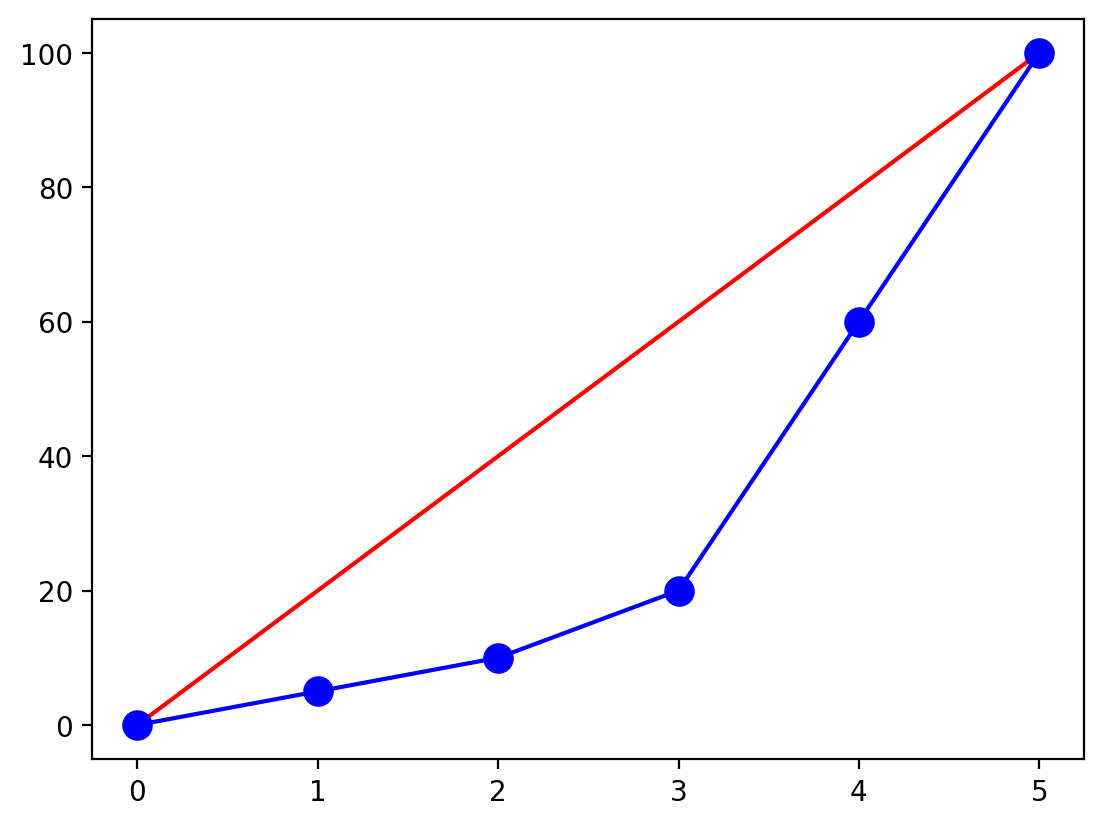
\includegraphics[scale=0.60]{img/exemple_courbe_lorenz_simple.png}
\end{center}

\bigskip

Encore plus visuellement, une fois la distribution ordonnée, on obtient donc $ 5 \; 5 \; 10 \; 40 \; 40 $.
L'histogramme suivant montre visuellement chaque valeur ajoutée entre les points de la courbe bleue.
Donc, en effectuant la somme des valeurs au fur et à mesure, chaque point de la courbe bleue correspond à $ 5 \; 10 \; 20 \; 60 \; 100 $.

\bigskip

\begin{center}
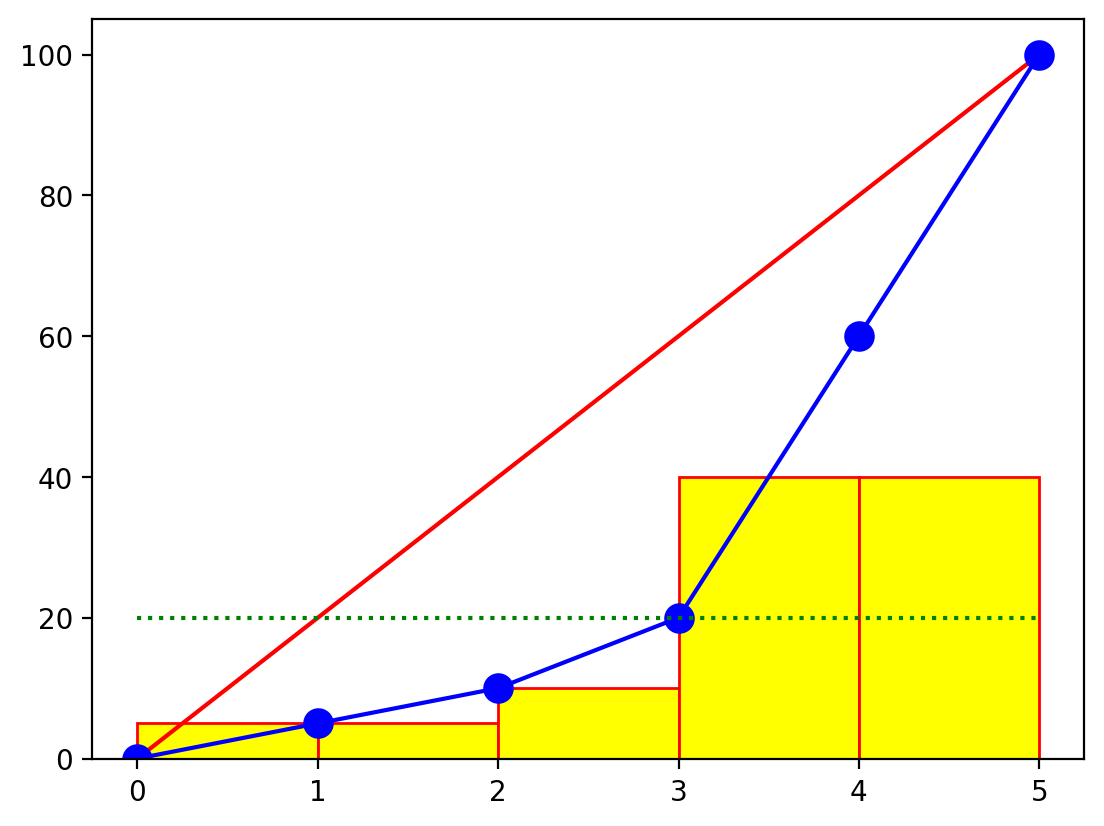
\includegraphics[scale=0.60]{img/exemple_courbe_lorenz-5-5-10-40-40.png}
\end{center}

\bigskip

Pour rappel, le coefficient de Gini correspond au double de l'aire entre la courbe bleue et la courbe rouge.
Pour bien apprécier visuellement l'écart de cette aire, prenons maintenant deux autres distributions, et comparons l'ensemble des cas :

\begin{itemize}
\item[$\bullet$] $ 0 \; 0 \; 0 \; 10 \; 90 $ (une distribution très inégale) : $ \text{Coeff Gini} = 0,760 $
\item[$\bullet$] $ 5 \; 5 \; 10 \; 40 \; 40 $ (une distribution plutôt inégale) : $ \text{Coeff Gini} = 0,424 $
\item[$\bullet$] $ 10 \; 15 \; 20 \; 25 \; 30 $ (une distribution peu inégale) : $ \text{Coeff Gini} = 0,200 $
\end{itemize}

Pour bien visualiser ces cas, la moyenne des distributions ($ 20 $) a été tracée en pointillés verts.

\begin{center}
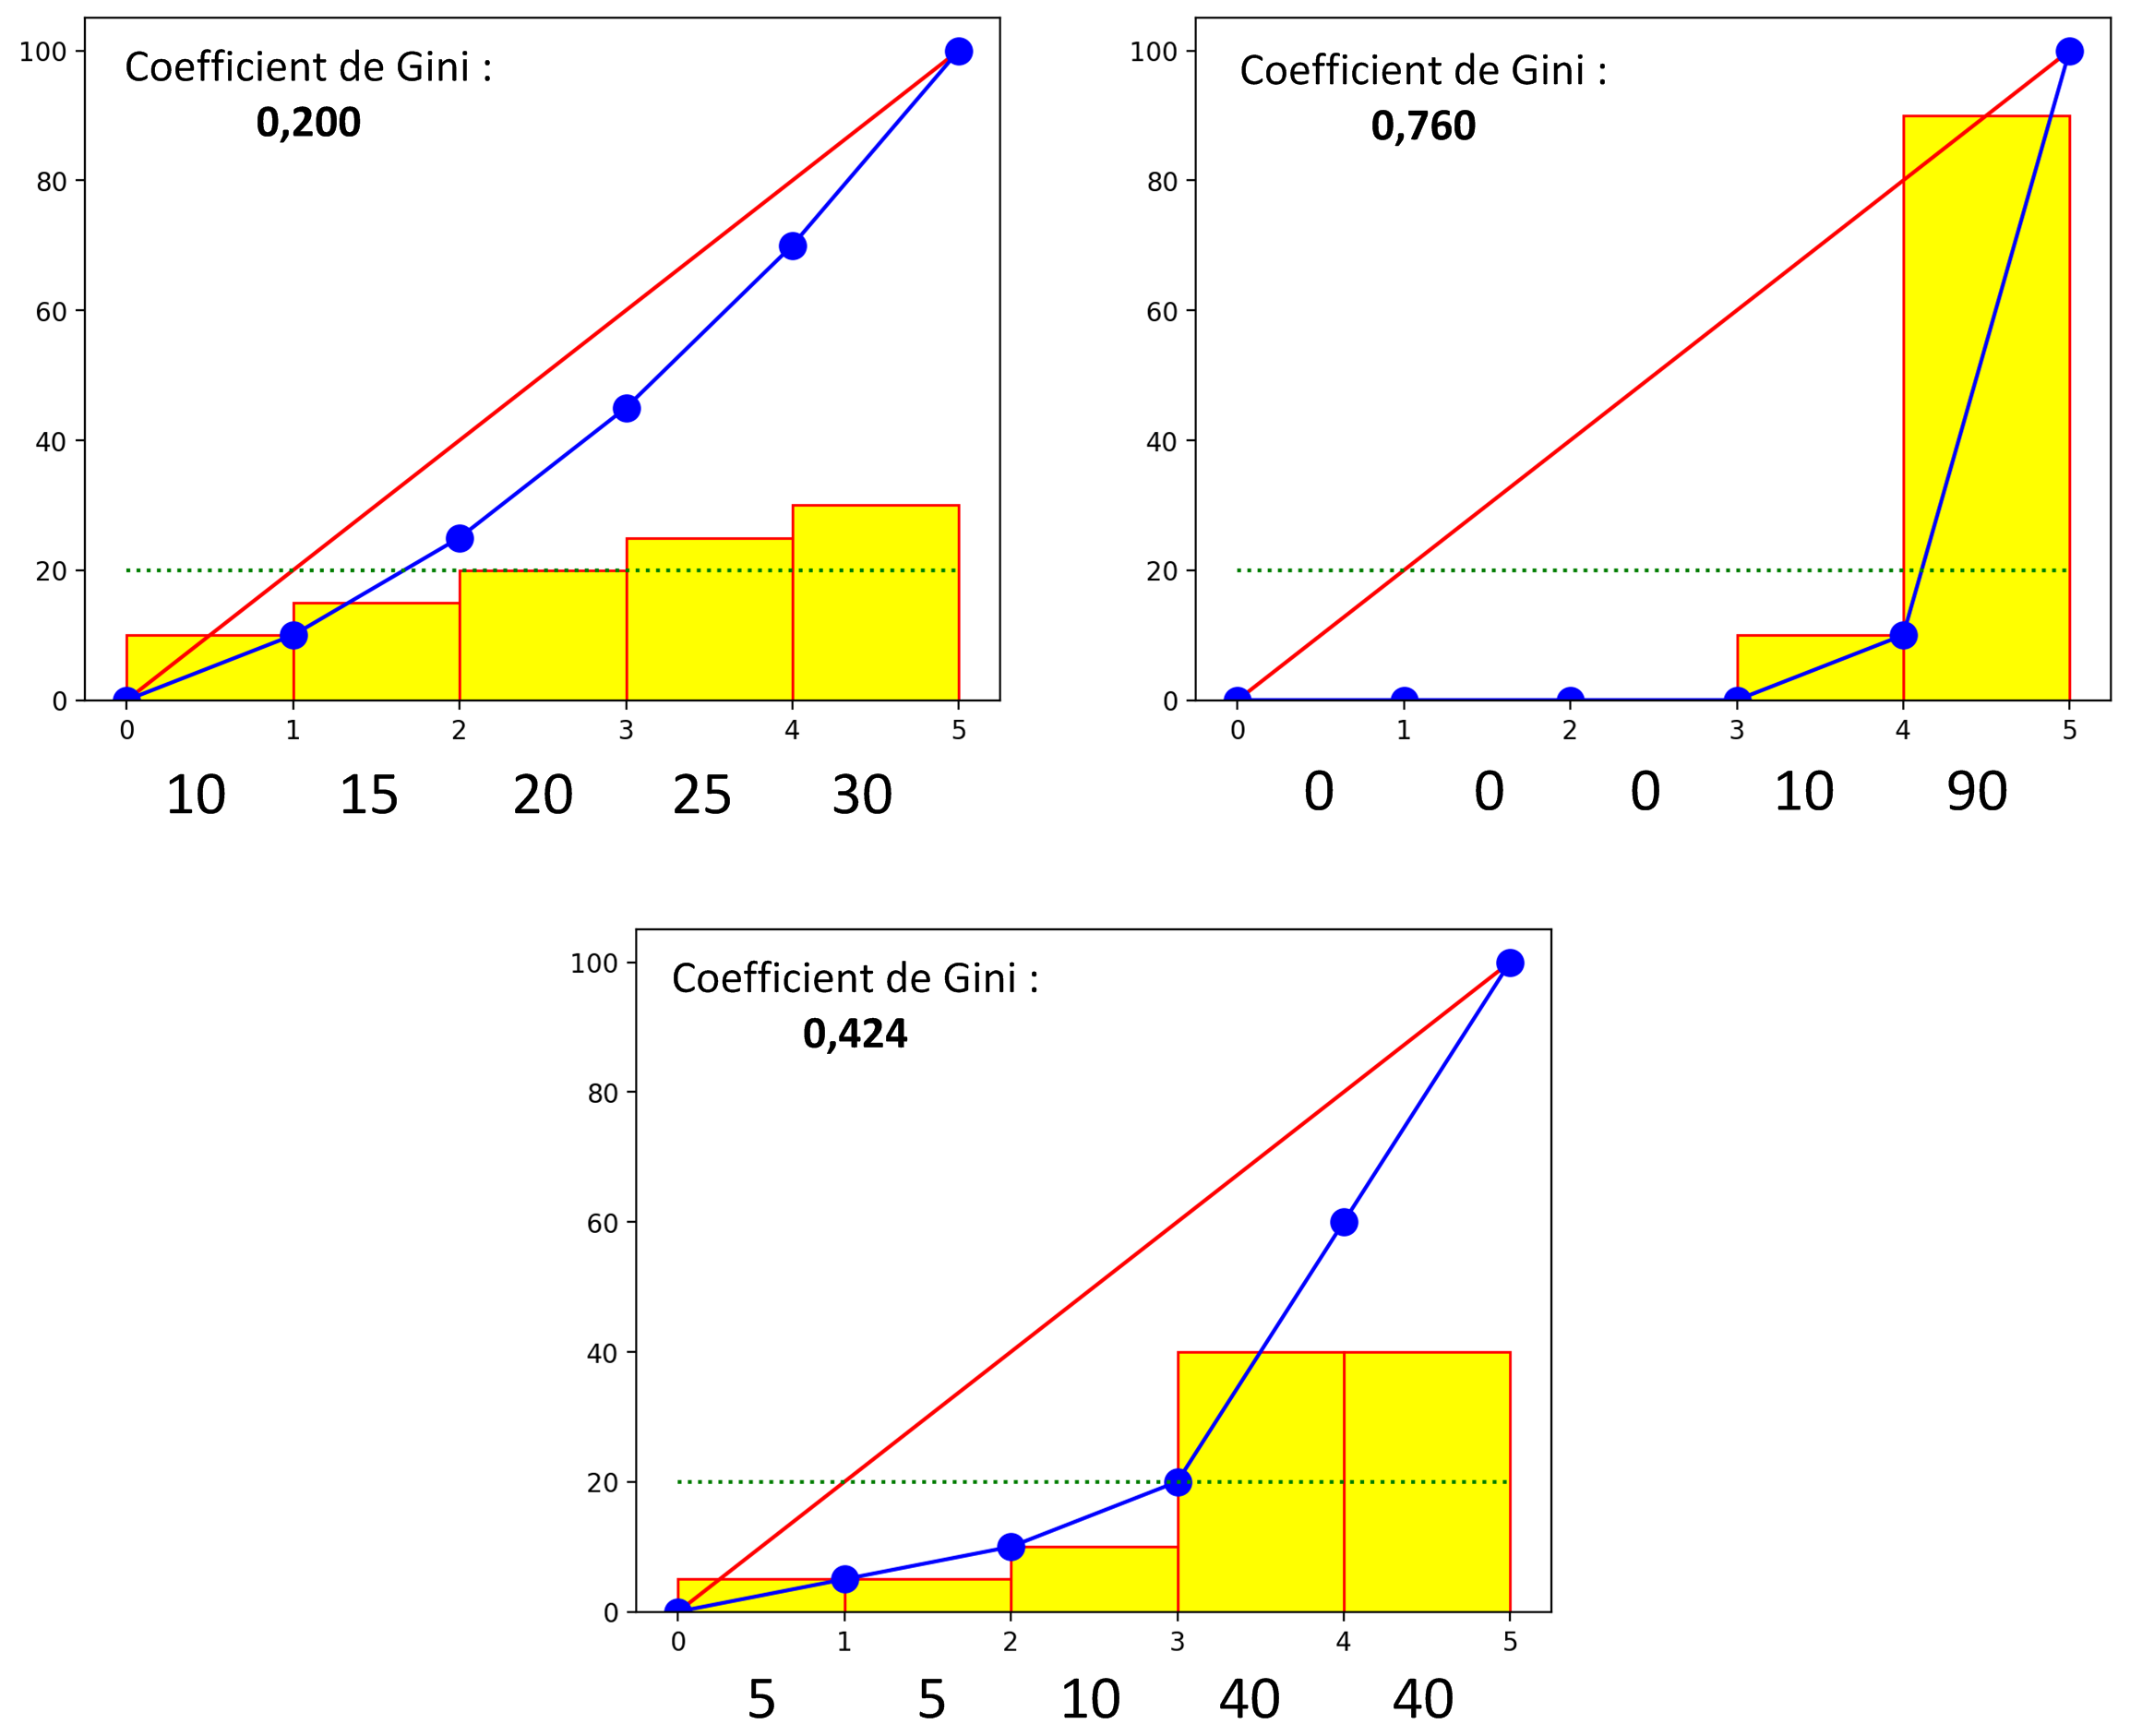
\includegraphics[scale=0.55]{img/exemple_courbes_lorenz.png}
\end{center}

Comme vous pouvez le constater, le cas peu inégal montre une courbe bleue proche de la courbe rouge, et inversement, le cas très inégal montre une courbe bleue très éloignée de la courbe rouge.
Pour rappel, la moyenne n'est pas un indicateur de dispersion, mais bien un indicateur de tendance centrale ou de position.
Les nombreux indicateurs que vous venez d'implémenter vous permettront donc de mieux interpréter les données dont vous disposerez dans votre carrière, et éventuellement de voir des phénomènes jusque-là peu visibles.

\bigskip

Reprenons l'implémentation du coefficient de Gini : vous venez de comprendre comment celui-ci est théoriquement construit et interprété.
Mais comment l'implémenter facilement ?

Deux formules nous intéressent particulièrement, la première est l'équation de Kendal et Stuart.
Dans celle-ci, $ n $ correspond au nombre d'éléments dans la distribution, et $ L_{1} , L_{2} , ... , L_{n} $ correspondent à chaque élément de la distribution.

\begin{center}
\begin{equation*}
G = \frac{ (1 / 2 n^{2}) \, \overset{n}{\underset{i = 1}{\sum}} \overset{n}{\underset{j = 1}{\sum}} \, | L_{i} - L_{j} | }{ (1 / n) \, \overset{n}{\underset{i = 1}{\sum}} \, L_{i}}
\end{equation*}
\end{center}

En observant cette formule, vous devriez remarquer que la double somme teste littéralement tous les éléments de la distribution deux à deux, ce qui est particulièrement long.
Et qu'il est par la suite nécessaire de diviser le tout par la somme des éléments.

\bigskip

Si vous implémentez chacune des parties indépendamment, le temps de calcul sera particulièrement long.
Et si vous implémenter toute la formule dans une fonction, vous aurez beaucoup de variables à conserver, et le code risque d'être difficile à comprendre.

\bigskip

Heureusement, vous devriez remarquer que le diviseur est constitué du nombre d'éléments de la distribution, et de leur somme... ce qui ressemble à la moyenne.
Et effectivement, Mookherjee et Shorrocks ont simplifié cette équation en introduisant la moyenne ($ \mu $) :

% G = \frac{ Moyenne des valeurs absolues des diff\acute{e}rences entre chaque Partie }{ Moyenne de toutes les Parties \times 2}
\begin{center}
\begin{equation*}
G = \frac{1}{2 \mu n^{2}} \, \overset{n}{\underset{i = 1}{\sum}} \overset{n}{\underset{j = 1}{\sum}} \, | L_{i} - L_{j} |
\end{equation*}
\end{center}
% Formule des trapèzes ou Formule des triangles ?
% = AE2 / (W2 * 2)
% AE2 = MOYENNE(ABS(L2-L2); ABS(L2-M2); ..... ; ABS(M2-L2); ABS(M2-M2); ....)
% W2 = MOYENNE(distribution)

Bien que cette formule semble encore complexe, décomposons-là :

\begin{itemize}
\item[$\bullet$] $ L_{i} - L_{j} $ correspond à la différence entre chaque élément de la distribution.

\item[$\bullet$] $ | L_{i} - L_{j} | $ correspond à la valeur absolue de la différence entre chaque élément de la distribution.

\item[$\bullet$] $ \overset{n}{\underset{i = 1}{\sum}} \overset{n}{\underset{j = 1}{\sum}} \, | L_{i} - L_{j} | $ correspond à la somme des différences absolues des éléments de la distribution. Il s'agit donc de faire une double boucle effectuant la différence entre chaque élément de la distribution, pour ajouter le résultat à une variable initialisée à $ 0 $ juste avant la boucle. La double boucle implique simplement d'itérer comme sur un tableau à deux dimensions ($ | L_{1} - L_{1} | + | L_{1} - L_{2} | + ... + | L_{2} - L_{1} | + | L_{2} - L_{2} | + ... + | L_{n} - L_{n} | $).

\item[$\bullet$] $  2 \mu n^{2} $ correspond simplement à $ 2 $ multiplié par la moyenne de la distribution, multiplié par la quantité d'éléments (le cardinal) au carré.
\end{itemize}


%def CoeffGini(MyDistribution):
%  DiffGini = 0
%  for i in MyDistribution:
%    for j in MyDistribution:
%      DiffGini = DiffGini + abs(i - j)
%  DiffGini = DiffGini / (DistrNbValues ** 2)
%  CoeffGini = DiffGini / (mean(MyDistribution) ** 2)
%  return (CoeffGini)


\newpage


\subsection{Statistiques sur distributions triées}

Les fonctions de ces exercices devront être écrites dans un fichier nommé \TTBF{my\_stats\_ordered.c} et leurs prototypes dans un fichier nommé \TTBF{my\_stats\_ordered.h} .


\question{Implémentez une fonction \TTBF{my\_sort} générant une version triée de la distribution donnée en paramètre. La nouvelle distribution \textit{doit} être distincte de celle donnée en paramètre : il faut pouvoir libérer indépendamment l'une sans affecter l'autre et vice versa.}

\begin{lstlisting}[language=C,morekeywords={floor,ceil}]
struct my_distribution *my_sort(struct my_distribution *distribution) \end{lstlisting}


\question{Implémentez une procédure \TTBF{my\_inplace\_sort} effectuant un tri en place de la distribution donnée en paramètre. Cette procédure déplace donc les valeurs dans la structure sans allouer de nouvelle structure intermédiaire.}

Pour rappel, n'hésitez pas à consulter les algorithmes vus dans les précédents cours (tri à bulles, tri par fusion, tri par insertion).

\medskip

\begin{lstlisting}[language=C,morekeywords={floor,ceil}]
void my_inplace_sort(struct my_distribution *distribution) \end{lstlisting}


\question{Implémentez une fonction \TTBF{my\_median} calculant la médiane de la distribution donnée en paramètre.}

Pour rappel, si la distribution a un nombre \textit{impair} de valeurs, alors on renvoie la valeur centrale, inversement, si la distribution a un nombre \textit{pair} de valeurs, alors on renvoie la moyenne des deux valeurs centrales.

\medskip

\begin{lstlisting}[language=C,morekeywords={floor,ceil}]
double my_median(struct my_distribution *distribution) \end{lstlisting}



\question{Implémentez plusieurs fonctions permettant de calculer l'écart interquartile de la distribution donnée en paramètre.}

Vous devrez implémenter les fonctions suivantes :

\begin{itemize}
\item \TTBF{my\_quartile\_zero} donnant l'index du quartile 0, \TTBF{my\_quartile\_one} donnant l'index du quartile 1, ..., \TTBF{my\_quartile\_four} donnant l'index du quartile 4
\item \TTBF{my\_get\_quartile} donnant l'index du quartile demandé (utilisez un \textit{switch ... case} pour appeler la bonne fonction). Si le quartile donné en paramètre n'existe pas, renvoyez $ -1 $
\item \TTBF{my\_inter\_quartile\_range} donnant l'écart interquartile
\end{itemize}


Parmi les mesures statistiques utiles se trouve l'\textit{écart interquartile} basé sur la différence entre des \textit{quartiles}.
L'idée des quartiles est de diviser la distribution en $ 4 $ parties, chaque quartile étant un séparateur, et d'observer l'écart entre certains séparateurs pour mesurer la dispersion des valeurs.

\begin{itemize}
\item le quartile 0 ($Q_{0}$) est la valeur la plus petite de la distribution
\item le $ 1^{er} $ quartile ($Q_{1}$) sépare les $ 25\% $ premières valeurs de la distribution des autres
\item le $ 2^{\grave{e}me} $ quartile ($Q_{2}$) sépare les $ 50\% $ premières valeurs de la distribution des autres
\item le $ 3^{\grave{e}me} $ quartile ($Q_{3}$) sépare les $ 75\% $ premières valeurs de la distribution des autres
\item le quartile 4 ($Q_{4}$) est la valeur la plus élevée de la distribution
\end{itemize}

\newpage

Plus visuellement, la distribution triée est séparée ainsi :

\begin{center}
$ Q_{0} $ ... (partie 1) ... $ Q_{1} $ ... (partie 2) ... $ Q_{2} $ ... (partie 3) ... $ Q_{3} $ ... (partie 4) ... $ Q_{4} $
\end{center}

Dans le cas dit \textit{discret} (c'est-à-dire non continu : on peut dénombrer les valeurs que l'on étudie), il suffit de calculer le \textit{rang} des valeurs, c'est-à-dire leur position dans la distribution triée par ordre croissant.
Un quartile dans le cas discret est donc simplement une valeur à une position précise dans la distribution triée.

\bigskip

Pour une distribution contenant $ n $ valeurs, on calcule les rangs ainsi :

\begin{itemize}
\item le quartile 0 ($Q_{0}$) est donc au rang $ 1 $
\item le $ 1^{er} $ quartile ($Q_{1}$) est au rang $ (n + 3) / 4 $
\item le $ 2^{\grave{e}me} $ quartile ($Q_{2}$) est au rang $ (n + 1) / 2 $ (il s'agit de la médiane)
\item le $ 3^{\grave{e}me} $ quartile ($Q_{3}$) est au rang $ (3n + 1) / 4 $
\item le quartile 4 ($Q_{4}$) est donc au rang $ n $
\end{itemize}

\bigskip

Testons sur la distribution : $ 1 \; 2 \; 3 \; 4 \; 5 \; 6 \; 7 \; 8 \; 9 $

\begin{itemize}
\item $ Q_{0} = 1 $
\item $ Q_{1} = 3 $
\item $ Q_{2} = 5 $
\item $ Q_{3} = 7 $
\item $ Q_{4} = 9 $
\end{itemize}

\bigskip

La première partie contient donc les valeurs de $ 1 \; 2 \; 3 $, la deuxième partie les valeurs de $ 3 \; 4 \; 5 $, la troisième partie les valeurs $ 5 \; 6 \; 7 $, et la quatrième partie les valeurs $ 7 \; 8 \; 9 $.

\smallskip

Si on ne tombe pas sur un rang précis, il est normalement nécessaire de calculer un poids entre la valeur au dessus et la valeur au dessous.
Mais pour simplifier notre cas, utilisons le rang inférieur (avec \TTBF{floor(3)}).

\bigskip

%\question{Créez cinq fonctions nommées \TTBF{QuartileZero}, \TTBF{QuartileOne}, \TTBF{QuartileTwo}, \TTBF{QuartileThree}, \TTBF{QuartileFour} calculant la valeur de chaque quartile pour une distribution donnée.}

\begin{lstlisting}[language=C,morekeywords={floor,ceil}]
int my_quartile_zero(struct my_distribution *distribution)
int my_quartile_one(struct my_distribution *distribution)
int my_quartile_two(struct my_distribution *distribution)
int my_quartile_three(struct my_distribution *distribution)
int my_quartile_four(struct my_distribution *distribution)

int my_get_quartile(struct my_distribution *distribution, int quartile) \end{lstlisting}

% Q0 = 1
% Q1 = (DistrNbValues + 3) / 4
% Q2 = DistrNbValues / 2
% Q3 = ((3 * DistrNbValues) + 1) / 4
% Q4 = DistrNbValues

\bigskip

Revenons à la métrique qui nous intéressait : l'écart interquartile.
Celui-ci se calcule simplement ainsi :

\begin{center} % \text{étendue} = \text{Valeur}_{\text{\textit{max}}} - \text{Valeur}_{\text{\textit{min}}}
\begin{equation*}
\text{écart interquartile} = EI = Q_{3} - Q_{1}
\end{equation*}
\end{center}

% EI = Q3 - Q1

\bigskip

\begin{lstlisting}[language=C,morekeywords={floor,ceil}]
double my_inter_quartile_range(struct my_distribution *distribution) \end{lstlisting}

\end{document}
